%!TEX root = ../template.tex
%%%%%%%%%%%%%%%%%%%%%%%%%%%%%%%%%%%%%%%%%%%%%%%%%%%%%%%%%%%%%%%%%%%%
%% chapter7.tex
%% NOVA thesis document file
%%
%% Chapter with the bioprinting system description.
%%%%%%%%%%%%%%%%%%%%%%%%%%%%%%%%%%%%%%%%%%%%%%%%%%%%%%%%%%%%%%%%%%%%
\chapter{Bioprinting System}
\label{cha:bioprinting_system}

\begin{quotation}
\begin{flushright}
\itshape
«Quotation»\\
\textbf{- Author}
\end{flushright}
\end{quotation}

The present chapter will fully describe the custom-made bioprinting system developed on this thesis.

First, a brief overview of the system will be presented. Next, the design guidelines will be mentioned. From there, the electronics and mechanical design are thoroughly described. Finally, it ends with an overview of the firmware and software developed for control. 

% ==========================
% = Overview =
% ==========================

\section{Overview}
\label{sec:bioprinting_system_overview}

The bioprinting system is composed by a custom-made robot end-effector that uses a syringe pump mechanism for bioink extrusion.

The goal of the system was to create an extrusion mechanism that could support the complete system by allowing a bioprint to be made. Because of this, it only uses a bioink volume of 10 \si{\milli\liter}. A full-fledged bioprinting system was not needed.

The extrusion mechanism is a lead screw directly attached to a stepper motor that drives the screw. The syringe plunger is attached to a lead screw allowing the movement of the latter to control the movement of the former. By turning the lead screw in each direction the syringe plunger moves inside or outside, pushing or sucking bioink.

The system can be controlled externally via wireless Bluetooth or through wired \gls{usb}. It is powered externally via a 12 \si{\volt} power source.

% section bioprinting_system_overview

% ==========================
% = Design Guidelines =
% ==========================

\section{Design Guidelines}
\label{sec:bioprinting_system_design_guidelines}

In order to conceive this system, various aspects needed to be addressed during the design phase. Some of the requirements for it were to:

\begin{itemize}
    \item be lightweight;
    \item avoid using external wired connections;
    \item be able to deal with a bioink viscosity up to 1 \si{\pascal\second};
\end{itemize}

These requirements impacted the selection of several components and processes like: the motor to drive the lead screw; the power source; and communication media.

To reduce external wired connections Bluetooth wireless communication was chosen for control. However, if needed, \gls{usb} connection is still available. The power source can also influence the presence of wires. For a complete wireless solution, 9 \si{\volt} batteries and 3.7 \si{\volt} \gls{lipo} batteries could be used. However, a 12 \si{\volt} external power source was chosen to simplify the design process. By not using batteries the total weight is also reduced.\\

The weight and viscosity were decisive criteria for the selection of the motor. Next, a calculation of the minimum torque needed by the motor is presented.

\subsection{Motor Torque Calculation}
\label{subsec:bioprinting_system_design_guidelines_torque_calculation}

For the torque calculation, a simplified syringe model was created to calculate the pressure at the plunger. The Poiseuille's law was used to calculate the pressure at each section of the syringe barrel. From that, the force at the plunger is obtained. Finally, using the lead screw model, the torque of the motor is calculated to supply the needed force. For this model gravity is not considered.\\

The Poiseuille's law (\ref{eq:poiseuille_law}), gives the pressure difference between two points along a long cylindrical pipe of constant cross section. This model law is only valid for incompressible and Newtonian fluids. In this equation, $\mu$ stands for the fluid viscosity; $L$ is the length of the pipe; $Q$ is the volumetric flow rate; and $R$ is the pipe radius. 

\begin{equation}
    \label{eq:poiseuille_law}
    \Delta p = \frac{8 \mu L Q}{\pi R^4}
\end{equation}

Based on the syringe model presented on Figure \ref{fig:syringe_model} and the respective values available on table \ref{tab:syringe_model_dimensions}, the force at the plunger calculated is rounded to 238 \si{\newton}. The fluid viscosity value used was 1 \si{\pascal\second} and the volumetric flow rate was 50 \si{\milli\liter\per\minute}. 

The calculation of the pressure difference on sections $L_{f1}$ and $L_{f2}$ used a diameter approximation. Since Poiseuille's law is valid for constant cross section, the mean value between the two diameters was used as the section diameter. \\

\begin{figure}[htbp]
	\centering
	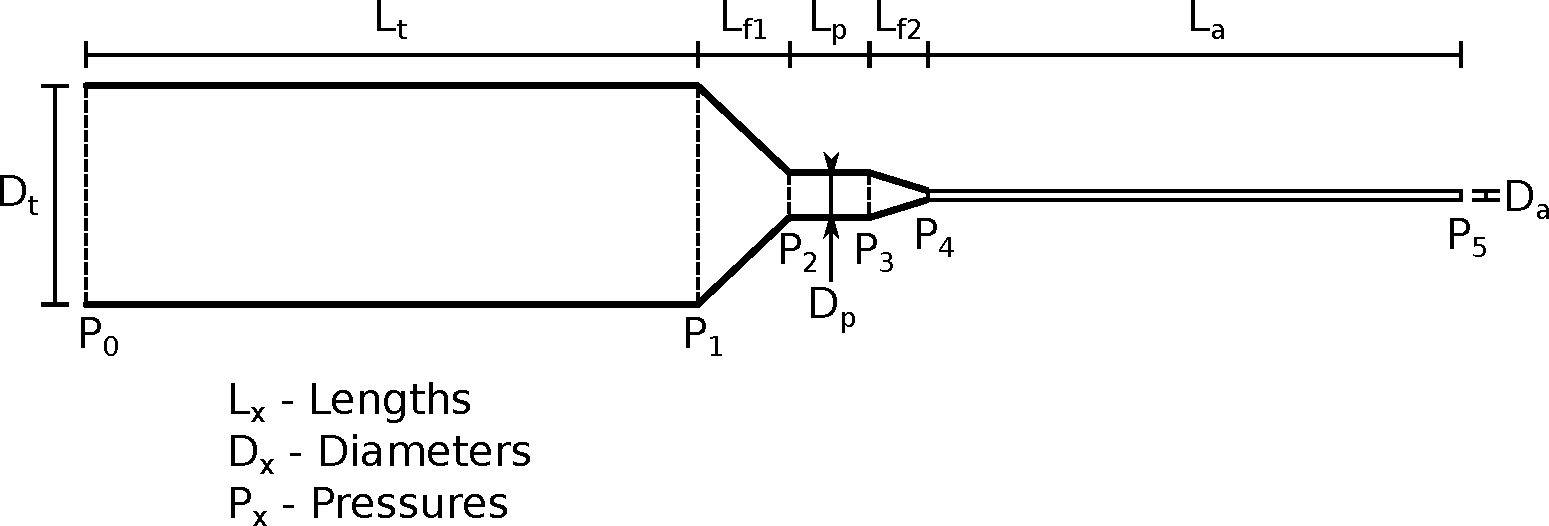
\includegraphics[width=\textwidth]{syringe_model}
	\caption{Syringe model used to calculate the force at the plunger need to push a 1 \si{\pascal\second} fluid at 50 \si{\milli\liter\per\minute}.}
	\label{fig:syringe_model}
\end{figure}

\begin{table}[htbp]
    \caption{Syringe model dimensions.}
    \centering
    \begin{threeparttable}
        \begin{tabular}{c|c|c|c|c|c|c|c|c}
        \toprule
             \textbf{Quantity} & $D_t$ & $D_p$ & $D_a$ & $L_t$ & $L_{f1}$ & $L_p$ & $L_{f2}$ & $L_a$ \\
        \midrule
             \textbf{Value} & 15.00 & 2.50 & 0.80 & 60.00 & 3.00 & 9.00 & 4.00 & 14.70 \\
        \bottomrule
        \end{tabular}
        \begin{tablenotes}
            \small
            \item \textbf{Notes:} All the values are in millimeters.
        \end{tablenotes}
    \end{threeparttable}
    \label{tab:syringe_model_dimensions}
\end{table}

To calculate the torque, the Lead Screw Lift/Lower Torque equations (\ref{eq:lead_screw_lift_torque}) (\ref{eq:lead_screw_lower_torque}) are used. $F$ is the load force that the mechanism needs to raise or lower. It corresponds to the force on the syringe plunger. The screw diameter corresponds to $d_m$. $l$ is the lead or screw pitch. $\mu$ is the friction coefficient between the screw and nut metals. Table \ref{tab:torque_calculation_dimensions} presents the values used.

The values calculated are rounded to 14 \si{\newton\centi\meter} (lift) and 8 \si{\newton\centi\meter} (lower).

\begin{equation}
    \label{eq:lead_screw_lift_torque}
    \tau = F \cdot \frac{d_m}{2} \left(\frac{l + \pi \cdot \mu \cdot d_m}{\pi \cdot d_m - \mu \cdot l}\right)  
\end{equation}

\begin{equation}
    \label{eq:lead_screw_lower_torque}
    \tau = F \cdot \frac{d_m}{2} \left(\frac{-l + \pi \cdot \mu \cdot d_m}{\pi \cdot d_m + \mu \cdot l}\right)  
\end{equation}

\begin{table}[htbp]
    \caption{Torque calculation parameters.}
    \centering
    \begin{threeparttable}
        \begin{tabular}{c|c|c|c|c}
        \toprule
             \textbf{Quantity} & $F$ & $d_m$ & $l$ & $\mu$ \\
        \midrule
             \textbf{Value} & 238 & 3.48 & 0.80 & 0.20 \\
        \midrule
             \textbf{Units} & \si{\newton} & \si{\milli\meter} & \si{\milli\meter} & - \\
        \bottomrule
        \end{tabular}
        \begin{tablenotes}
            \small
            \item \textbf{Notes:} Some of the values used are approximations.
        \end{tablenotes}
    \end{threeparttable}
    \label{tab:torque_calculation_dimensions}
\end{table}

Based on the torque value obtained, the motor selected was a NEMA17 stepper motor which has 42 \si{\newton\centi\meter} holding torque. The torque of this motor is three times higher that the calculated value. This provides a high margin for any model limitations related to model simplification. The motor characteristics will be presented on sections \ref{sec:bioprinting_system_electronics_design} and \ref{sec:bioprinting_system_mechanical_design}.

% subsection bioprinting_system_design_guidelines_torque_calculation

% section bioprinting_system_design_guidelines

% ==========================
% = Electronics Design =
% ==========================

\section{Electronics Design}
\label{sec:bioprinting_system_electronics_design}

The present section aims to describe the electronics design of the bioprinting system. It will detail the components list, present the schematics and the \gls{pcb}. It will end with the system's electrical characteristics. The electronics block diagram is presented on Figure \ref{fig:bioprinting_electronics_block_diagram}.

\begin{figure}[htbp]
	\centering
	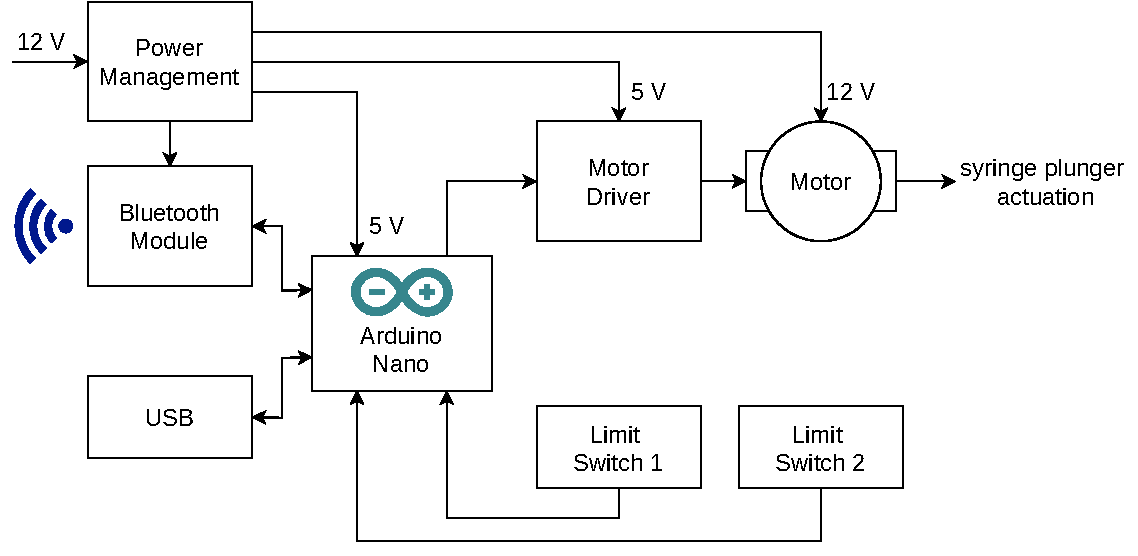
\includegraphics[width=\textwidth]{bioprinting_electronics_block_diagram}
	\caption{Bioprinting system's electronics block diagram. The system is controlled by an Arduino Nano. This interfaces the motor through a motor controller which simplifies the control algorithm. The Arduino communicates with the rest of the main system via Bluetooth or \gls{usb}. Two limit switches notify the Arduino when the syringe plunger reaches the lead screw limits. A power management unit is responsible for supplying the necessary voltage and current to the various components.}
	\label{fig:bioprinting_electronics_block_diagram}
\end{figure}

\subsection{Bill of Materials}
\label{subsec:bioprinting_system_electronics_design_bom}

The electronics of the bioprinting system consists of six main components: an Arduino Nano Rev3; an A4988 motor driver; a NEMA17 stepper motor; an HC-06 Bluetooth module; and two lever limit switches. Besides these main six, the circuit has are other smaller electronic components that will be listed on the \gls{bom}, table \ref{tab:bom}.\\

The Arduino Nano acts as the brain of the system. It provides a \gls{usb} interface for programming and communication. It connects with the Bluetooth module via \gls{usart} for communication with the main Control System running on a computer.

Two limit switches connect to digital pins on the Arduino. They act as mechanical sensors that detect when the syringe plunger reaches the limits of the lead screw. This notification is important to stop the motor whenever it happens.

The main goal of the Arduino is to control the stepper motor. To simplify this control, an A4988 motor driver breakout board is used. This \gls{ic}, A4988, provides several microstepping modes that allows fine motor step control. It has an interface for microcontrollers and to connect the motor.\\

For more information about the main electronic components see the annex \ref{ann:bioprinting_system_datasheets}. It provides datasheets and reference documents for these components.

\begin{table}[htbp]
    \resizebox{\textwidth}{!}{%
    \begin{threeparttable}
        \caption{Electronics Bill of Materials.}
        \centering
        \begin{tabular}{c|l|c|c|c}
        \toprule
             \textbf{Number} & \textbf{Name} & \textbf{Reference} & \textbf{Value} & \textbf{Quantity} \\
        \midrule
             1 & Arduino Nano Rev3 & - & ATmega328 & 1 \\
             2 & Motor Driver & - & A4988 & 1 \\
             3 & Bluetooth Module & - & HC-06 & 1 \\
             4 & Micro Lever Limit Switch & - & - & 2 \\
             5 & NEMA17 Stepper Motor & - & 17HS4401 & 1 \\
        \bottomrule
        \end{tabular}
        \begin{tablenotes}
            \small
            \item \textbf{Notes:} The reference column corresponds to component codes defined on the schematics and \gls{pcb}. The value column can have the component part code or the electrical value.
        \end{tablenotes}
        \label{tab:bom}
    \end{threeparttable}}
\end{table}

% subsection bioprinting_system_electronics_design_bom

\subsection{Schematics}
\label{subsec:bioprinting_system_electronics_design_schematics}

The electronic schematic was created using the open source \gls{eda} suite KiCad \cite{KiCad_webpage}. The Eeschema application is the one used for schematic design. This sections presents the schematic in blocks. For the full page schematic, refer to appendix \ref{app:print_head_electronic_mechanical_design_files}.

% subsection bioprinting_system_electronics_design_schematics

\subsection{Printed Circuit Board}
\label{subsec:bioprinting_system_electronics_design_pcb}

The \gls{pcb} was also designed on KiCad, using Pcbnew application. The goal of the \gls{pcb} was to create a single board to aggregate the Arduino, the motor driver and the power management block. A single board will reduce the wiring, compact the design and ease the assembly process.

This sections only presents a close up of the \gls{pcb} (Fig. \ref{fig:print_head_pcb}). For the full page \gls{pcb}, refer to appendix \ref{app:print_head_electronic_mechanical_design_files}.

\begin{figure}[htbp]
	\centering
	\includegraphics[width=\textwidth]{print_head_pcb}
	\caption{Print Head printed circuit board.}
	\label{fig:print_head_pcb}
\end{figure}

% subsection bioprinting_system_electronics_design_pcb

\subsection{Electrical Characteristics}
\label{subsec:bioprinting_system_electronics_characteristics}

To properly define the electronics of the print head, the absolute maximum ratings and general electrical characteristics are presented on tables  \ref{tab:print_head_max_ratings} and \ref{tab:print_head_electric_characteristics}, respectively.

\begin{table}[htbp]
    \caption{Absolute Maximum Ratings.}
    \centering
    \begin{threeparttable}
        \begin{tabular}{l|c|c|c|c}
        \toprule
             \textbf{Characteristic} & \textbf{Symbol} & \textbf{Notes} & \textbf{Rating} & \textbf{Units} \\
        \midrule
             & & & & \\
        \bottomrule
        \end{tabular}
        \begin{tablenotes}
            \small
            \item \textbf{Notes:} ...
        \end{tablenotes}
    \end{threeparttable}
    \label{tab:print_head_max_ratings}
\end{table}

\begin{table}[htbp]
    \caption{Electrical Characteristics.}
    \centering
    \begin{threeparttable}
        \begin{tabular}{l|c|c|c|c|c}
        \toprule
              \textbf{Characteristic} & \textbf{Symbol} & \textbf{Min.} & \textbf{Typ.} & \textbf{Max.} & \textbf{Units} \\
        \midrule
             & & & & & \\
        \bottomrule
        \end{tabular}
        \begin{tablenotes}
                \small
                \item \textbf{Notes:} ...
            \end{tablenotes}
    \end{threeparttable}
    \label{tab:print_head_electric_characteristics}
\end{table}

% subsection bioprinting_system_electronics_characteristics

% section: bioprinting_system_electronics_design

% ==========================
% = Mechanical Design =
% ==========================

\section{Mechanical Design}
\label{sec:bioprinting_system_mechanical_design}

There exist several different thread types for lead screws. The chosen screw is a M8 standard screw. The thread type is an ISO metric thread. It consists of a symmetric V-shaped thread (Fig. \ref{fig:iso_thread_shape}).\\

\begin{figure}[htbp]
	\centering
	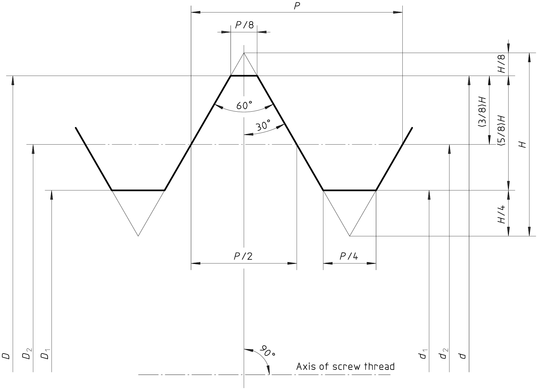
\includegraphics[width=.8\textwidth]{iso_thread_shape.png}
	\caption{ISO 68-1:1998 metric screw threads basic profile. Courtesy of International Standards Organization and adapted from \cite{ISO1998_metric_lead_screw_threads}.}
	\label{fig:iso_thread_shape}
\end{figure}

% section: bioprinting_system_mechanical_design

% ==========================
% = Firmware & Software =
% ==========================

\section{Firmware \& Software}
\label{sec:bioprinting_system_fw_sw}

% section: bioprinting_system_fw_sw